\documentclass{beamer}
\usepackage[fontset=adobe]{ctex}
\usetheme{Boadilla}
\setbeamercovered{dynamic}
\beamertemplatenavigationsymbolsempty
\title{基于公众关注度的股票市场的分析与预测}
\subtitle{综合论文训练答辩}
\author{李雨田}
\institute{清华大学}
\begin{document}

\begin{frame}
\titlepage
\begin{center}
  \begin{tabular}{ll}
    指导老师 & 余宏亮 \\
    报告人 & 李雨田 \\
    学号 & 2010012193
  \end{tabular}
\end{center}
\end{frame}

\begin{frame}{数据获取及预处理}{目的}
\begin{itemize}
  \item 统一数据结构
  \pause
  \item 高效率
  \pause
  \item 易用
\end{itemize}
\end{frame}

\begin{frame}{数据获取及预处理}{框架}
\begin{itemize}
  \item 基于 JSON 和 Redis 数据库
  \pause
  \item 基于事件循环机制
  \pause
  \item 提供 JavaScript 和 Python 库,与 Numpy , Pandas 和 StatsModels 对接
\end{itemize}
\end{frame}

\begin{frame}{数据来源}
\begin{itemize}
  \item 挑选上证 50 指数成分股
  \pause
  \item 从东方财富网股吧获取用户关注度数据
  \begin{itemize}
    \item 个股所有讨论帖点击量
    \item 对应的时间和内容
  \end{itemize}
  \pause
  \item 从国信证券客户端获取历史股票价格和交易量
\end{itemize}
\end{frame}

\begin{frame}{数据来源}{示例}
\begin{figure}
  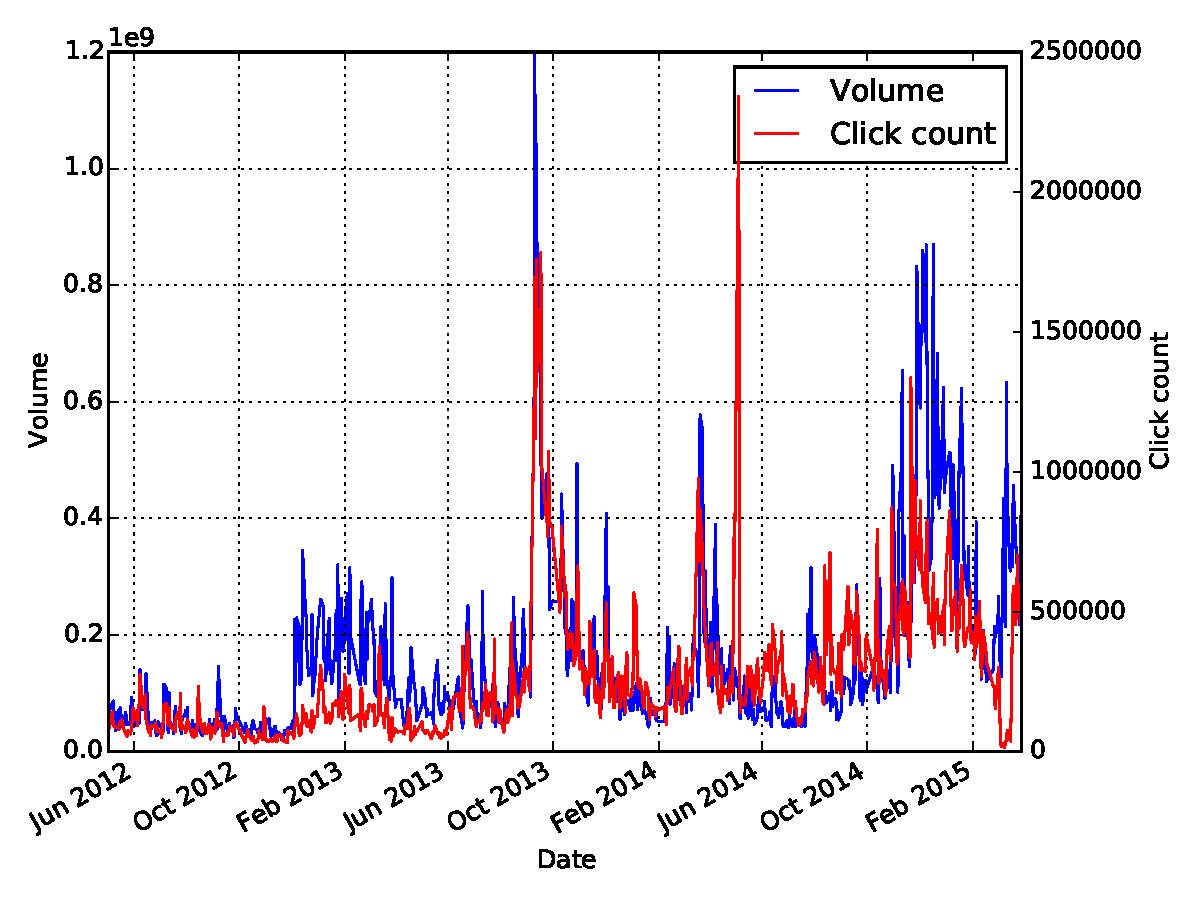
\includegraphics[width=0.6\textwidth]{plots/volume_and_click_count.pdf}
  \caption{浦发银行 (600000) 成交量与讨论帖点击量关系}
\end{figure}
\end{frame}

\begin{frame}{数据来源}{示例}
\begin{figure}
  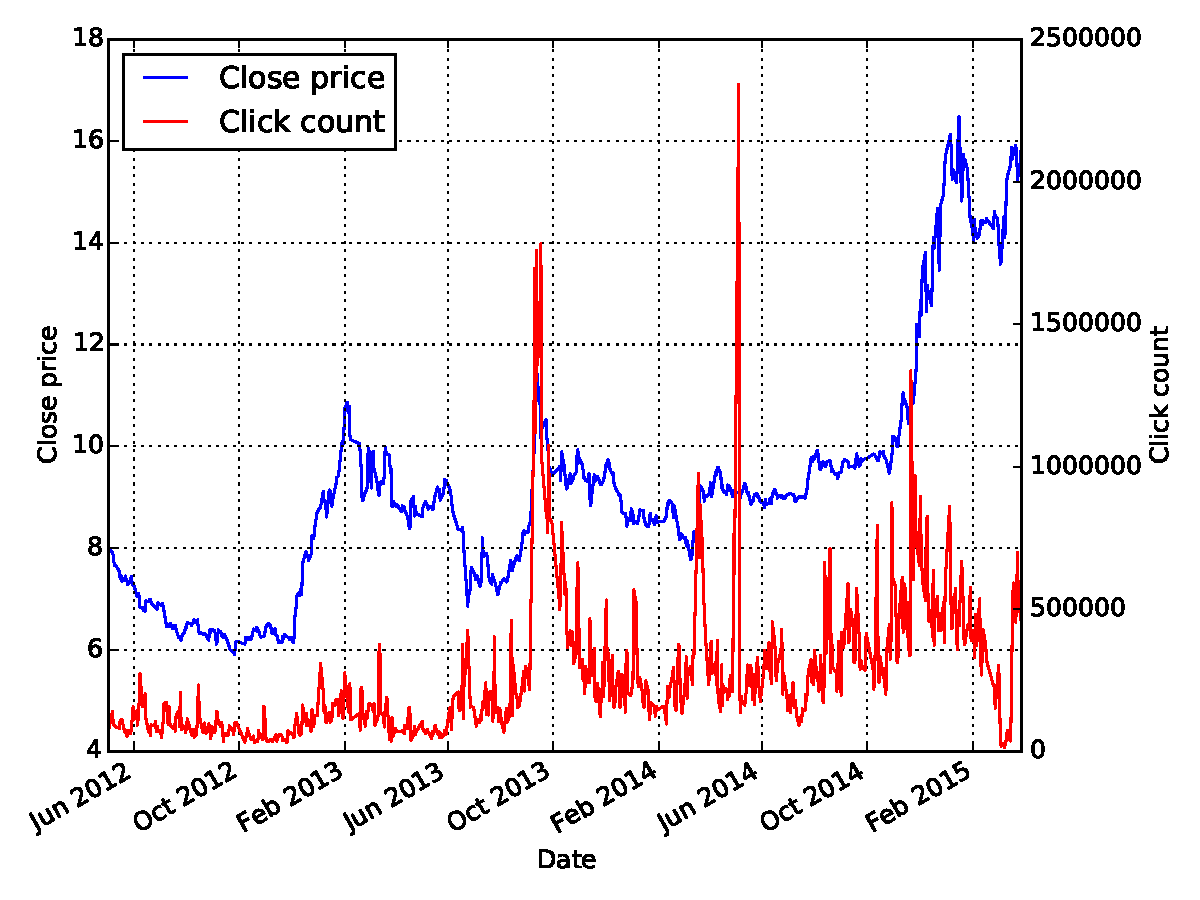
\includegraphics[width=0.6\textwidth]{plots/price_and_click_count.pdf}
  \caption{浦发银行 (600000) 价格与讨论帖点击量关系}
\end{figure}
\end{frame}

\begin{frame}{情感分析}
\begin{itemize}
  \item 拼接讨论帖标题和内容,去除非中文字符,使用翻译 API 翻译成英文
  \pause
  \item 使用卷积神经网络分析情感,该模型基于 Twitter 数据训练得到
\end{itemize}
\end{frame}

\begin{frame}{情感分析}
\begin{figure}
  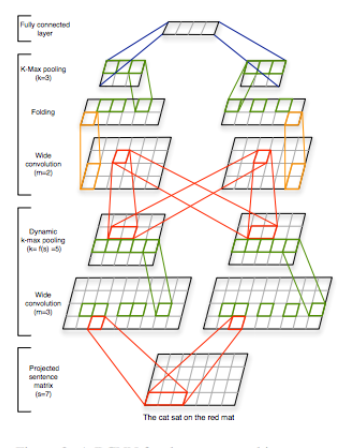
\includegraphics[width=0.4\textwidth]{plots/0.png}
  \caption{情感分析卷积神经网络}
\end{figure}
\end{frame}

\begin{frame}{因果关系分析}{格兰杰因果关系}
\begin{block}{假设检验}
  \[
    y_{t}=a_{0}+\sum_{i=1}^{m}a_{i}y_{t-i}+\sum_{i=1}^{m}b_{i}x_{t-i}+residual_{t}
  \]
  \[
    H_{0}:b_{1}=b_{2}=\cdots =b_{m}=0
  \]
\end{block}
\end{frame}

\begin{frame}{因果关系分析}{结果}
\begin{figure}
  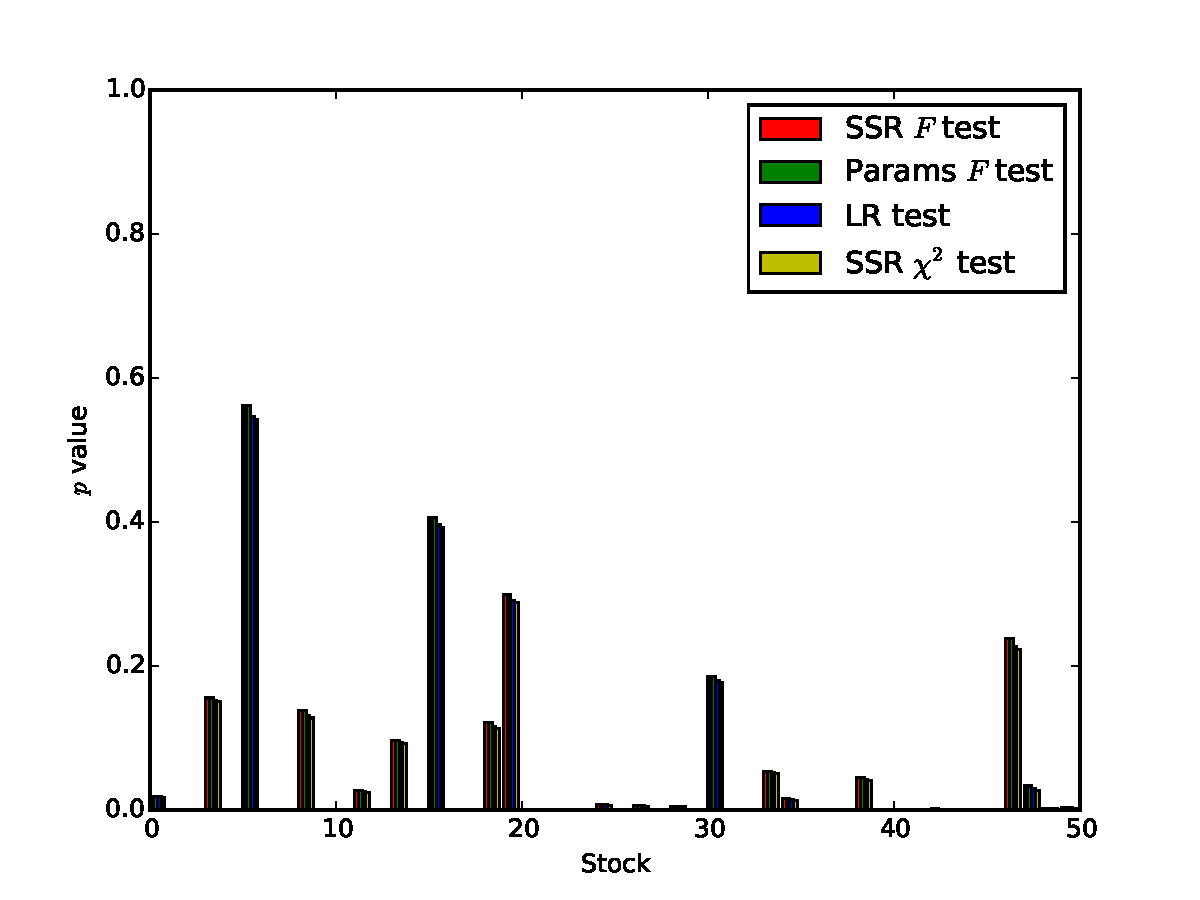
\includegraphics[width=0.6\textwidth]{plots/granger_causality_test_volume_on_sse_50.pdf}
  \caption{上证 50 成交量与讨论帖点击量格兰杰因果关系检验}
\end{figure}
\end{frame}

\begin{frame}{因果关系分析}{结果}
\begin{figure}
  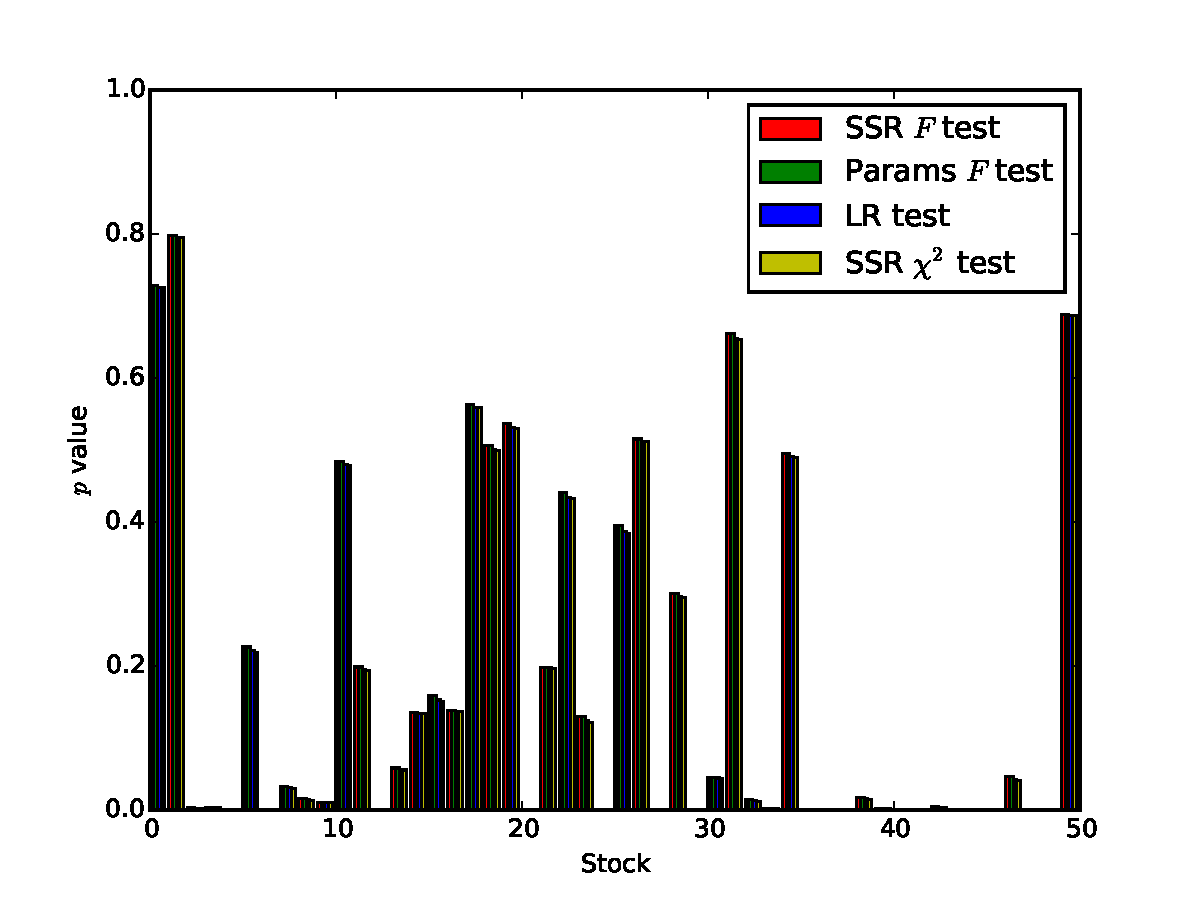
\includegraphics[width=0.6\textwidth]{plots/granger_causality_test_price_on_sse_50.pdf}
  \caption{上证 50 价格与讨论帖点击量格兰杰因果关系检验}
\end{figure}
\end{frame}

\begin{frame}{因果关系分析}{结果}
\begin{figure}
  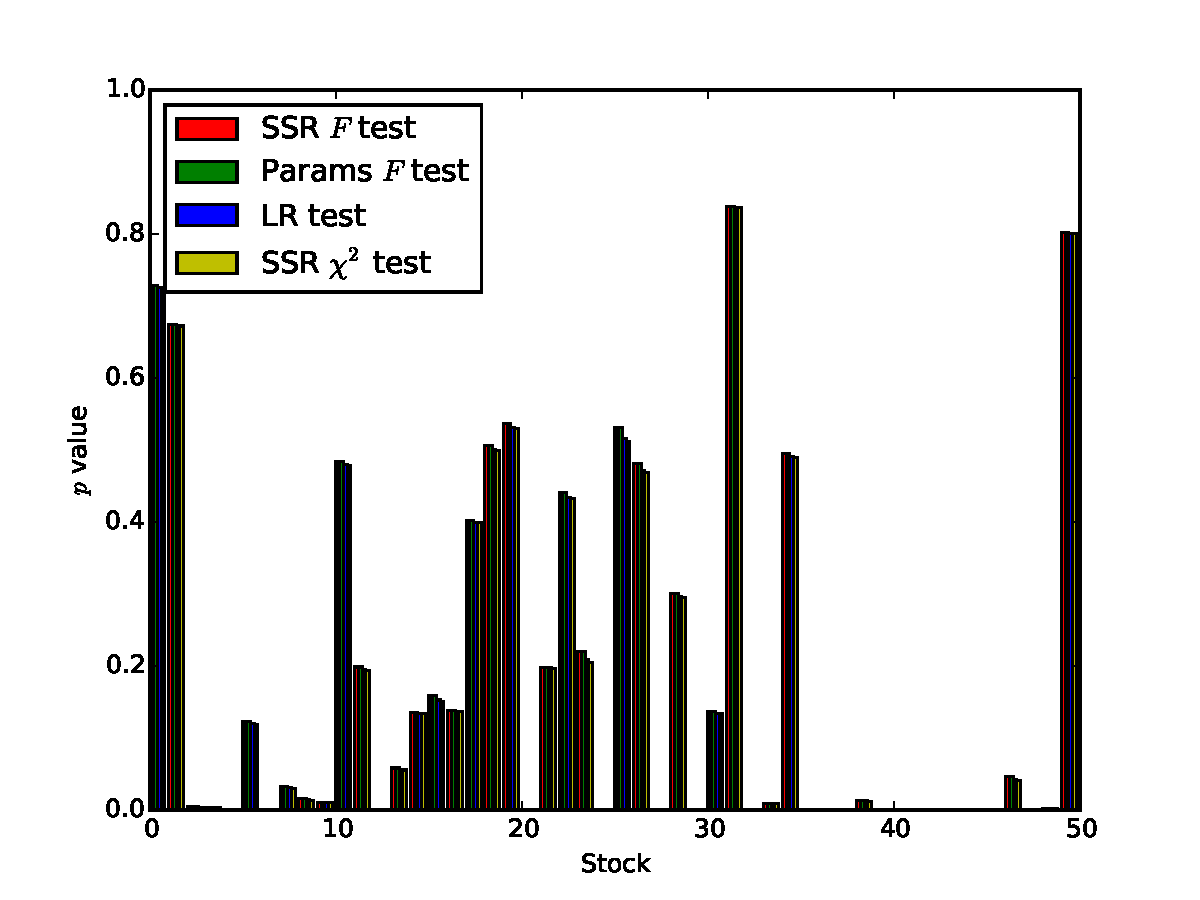
\includegraphics[width=0.6\textwidth]{plots/granger_causality_test_price_positive_on_sse_50.pdf}
  \caption{上证 50 价格与积极讨论帖点击量格兰杰因果关系检验}
\end{figure}
\end{frame}

\begin{frame}{预测模型}{向量自回归模型}
\begin{block}{定义}
  \[
    y_{t}=c+A_{1}y_{t-1}+A_{2}y_{t-2}+\cdots +A_{p}y_{t-p}+e_{t}
  \]
\end{block}
\end{frame}

\begin{frame}{预测模型}{框架}
\begin{itemize}
  \item 数据预处理
  \pause
  \begin{itemize}
    \item 计算量比
  \end{itemize}
  \pause
  \item 落后期选择
  \pause
  \begin{itemize}
    \item Akaike information criterion
    \pause
    \item Bayesian information criterion
    \pause
    \item Final prediction error
    \pause
    \item Hannan-Quinn information criterion
  \end{itemize}
  \pause
  \item 步长选择
\end{itemize}
\end{frame}

\begin{frame}{预测模型}{结果}
\begin{block}{定义}
  \[
    \operatorname{RMSE}=\sqrt{\frac{\sum_{i=1}^{n}(\hat{y}_{i}-y_{i})^{2}}{n}}
  \]
  \[
    \operatorname{NRMSE}=\frac{\operatorname{RMSE}}{y_{max}-y_{min}}
  \]
\end{block}
\end{frame}

\begin{frame}{预测模型}{结果}
以下结果中有 $NRMSE=5.857\times 10^{-2}$ 。

\begin{figure}
  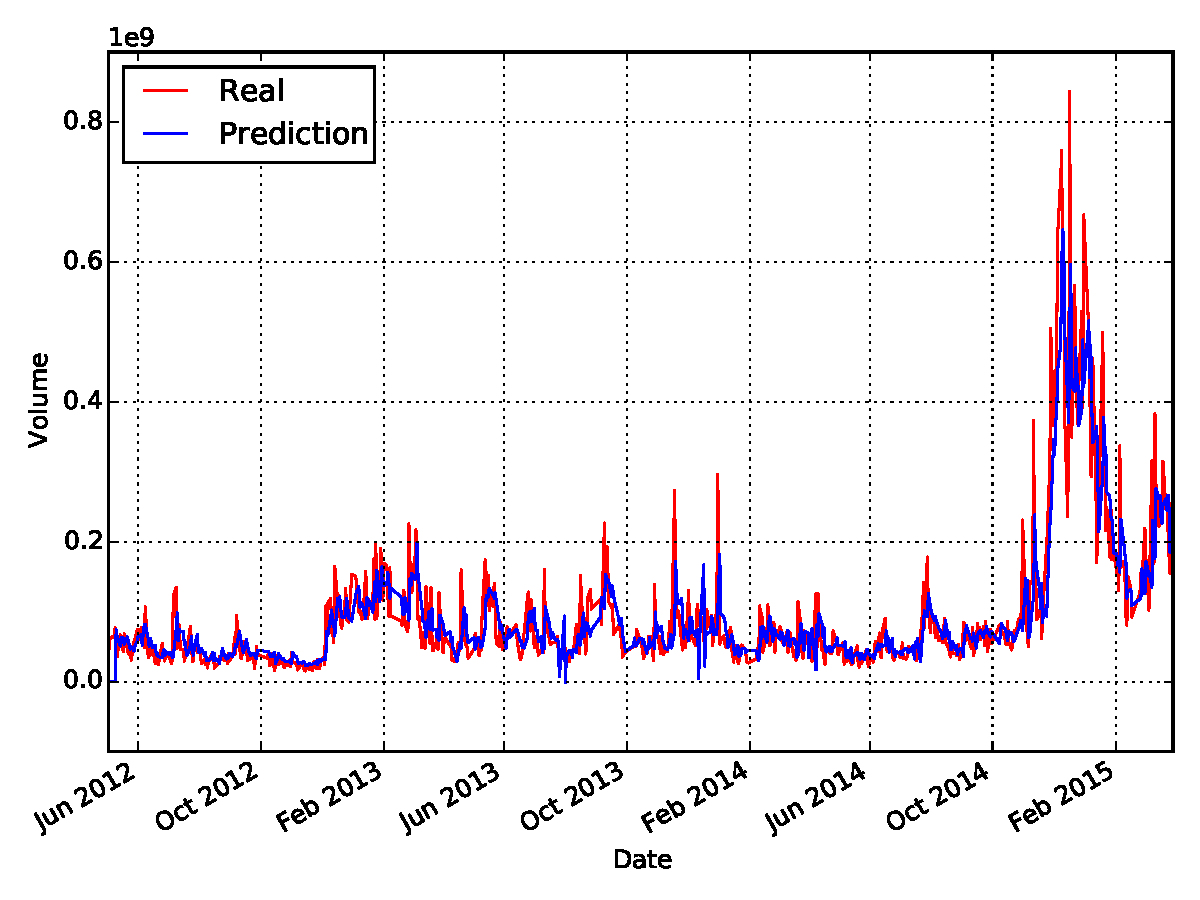
\includegraphics[width=0.6\textwidth]{plots/volume_forecast_regression_line.pdf}
  \caption{招商银行 (600036) 成交量预测}
\end{figure}
\end{frame}

\begin{frame}{预测模型}{结果}
以下结果中有 $NRMSE=2.546\times 10^{-2}$ 。

\begin{figure}
  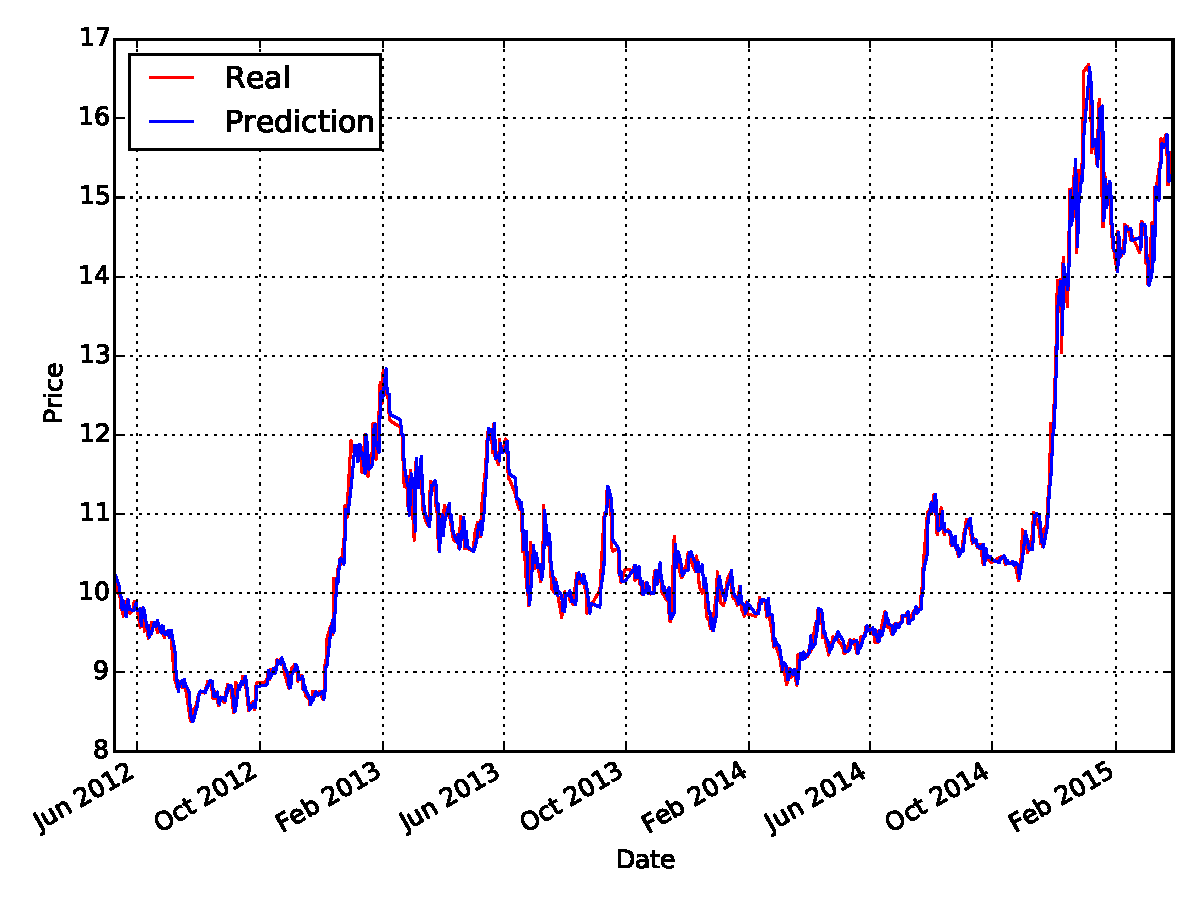
\includegraphics[width=0.6\textwidth]{plots/price_forecast_regression_line.pdf}
  \caption{招商银行 (600036) 价格预测}
\end{figure}
\end{frame}

\begin{frame}
\begin{center}
  \Huge 谢谢
\end{center}
\end{frame}

\end{document}
